\chapter{Full CLs Shape-Based Limits
\label{ch:limits}}

Null hypothesis $H_{0}$ : $b$, background-only \\
Alternate hypothesis $H_{1}$ : $s+b$, signal + background

We define $\mathcal{P}(\theta; N_{H_{i}})$ as the Poisson probability to observe $\theta$ events in data given the hypothesis $H_{i}$ which predicts $N_{H_{i}}$ events. This probability can be defined generally for the whole sample, but also per bin for a histogram of some quantity, e.g. $S_{T}$, and/or per channel.

In addition to that, we also need to consider the nuisance parameters:
\begin{equation}
\mathcal{P}(N_H,\theta) = \int \mbox{Poisson}(\theta; N_{H},\eta)f(\eta)d\eta
\end{equation}
where $f$ is the pdf for the nuisance parameter $\eta$, and the expression is integrated over all parameters.

With those definitions, we can write the test statistic $\mathcal{Q}$ as a ratio of likelihoods for a basic cut and count experiment:
\begin{equation}
\mathcal{Q} = \frac{\mathcal{P}(\theta; N_{H_{1}})}{\mathcal{P}(\theta; N_{H_{0}})}
\end{equation}
Splitting into bins and channel gives us:
\begin{equation}
\mathcal{Q} = \prod_{i=e,\mu}\prod_{j=0}^{n_{\text{bin}}} \frac{\mathcal{P}_{i,j}(\theta; N_{H_{1}})}{\mathcal{P}_{i,j}(\theta; N_{H_{0}})}
\end{equation}

Note: for simplicity of computation, we can define and use the log likelihood ratio:
\begin{equation}
q = -2 \ln \mathcal{Q}
\end{equation}

We perform several pseudo-experiments for each hypothesis by varying $\theta$ and keep the $\mathcal{Q}$ (or $q$) value for each hypothesis and pseudo-experiment. Finally, we compute the same for $\theta=N_{\text{obs}}$ to get $\mathcal{Q}_{\text{obs}}$.
The $CL_{s+b}$ and $CL_{b}$ variables correspond to the probability to get an observed $\mathcal{Q}$ greater than the $\mathcal{Q}$ obtained for the hypotheses $H_1$ and $H_0$. When using $q$, the observed value should be smaller than the value for the hypothesis. A visual example of these variables is shown in Fig. \ref{fig:q}.
\begin{align}
CL_{s+b} &= \mathcal{P}(\mathcal{Q} \leq \mathcal{Q}_{obs}|H_1) = \mathcal{P}(q \geq q_{obs}|H_1) \\
CL_{b} &= \mathcal{P}(\mathcal{Q} \leq \mathcal{Q}_{obs}|H_0) = \mathcal{P}(q \geq q_{obs}|H_0) \\
CL_{s} &= CL_{s+b}/CL_{b}
\end{align}

\begin{figure}[htbp]
\begin{center}
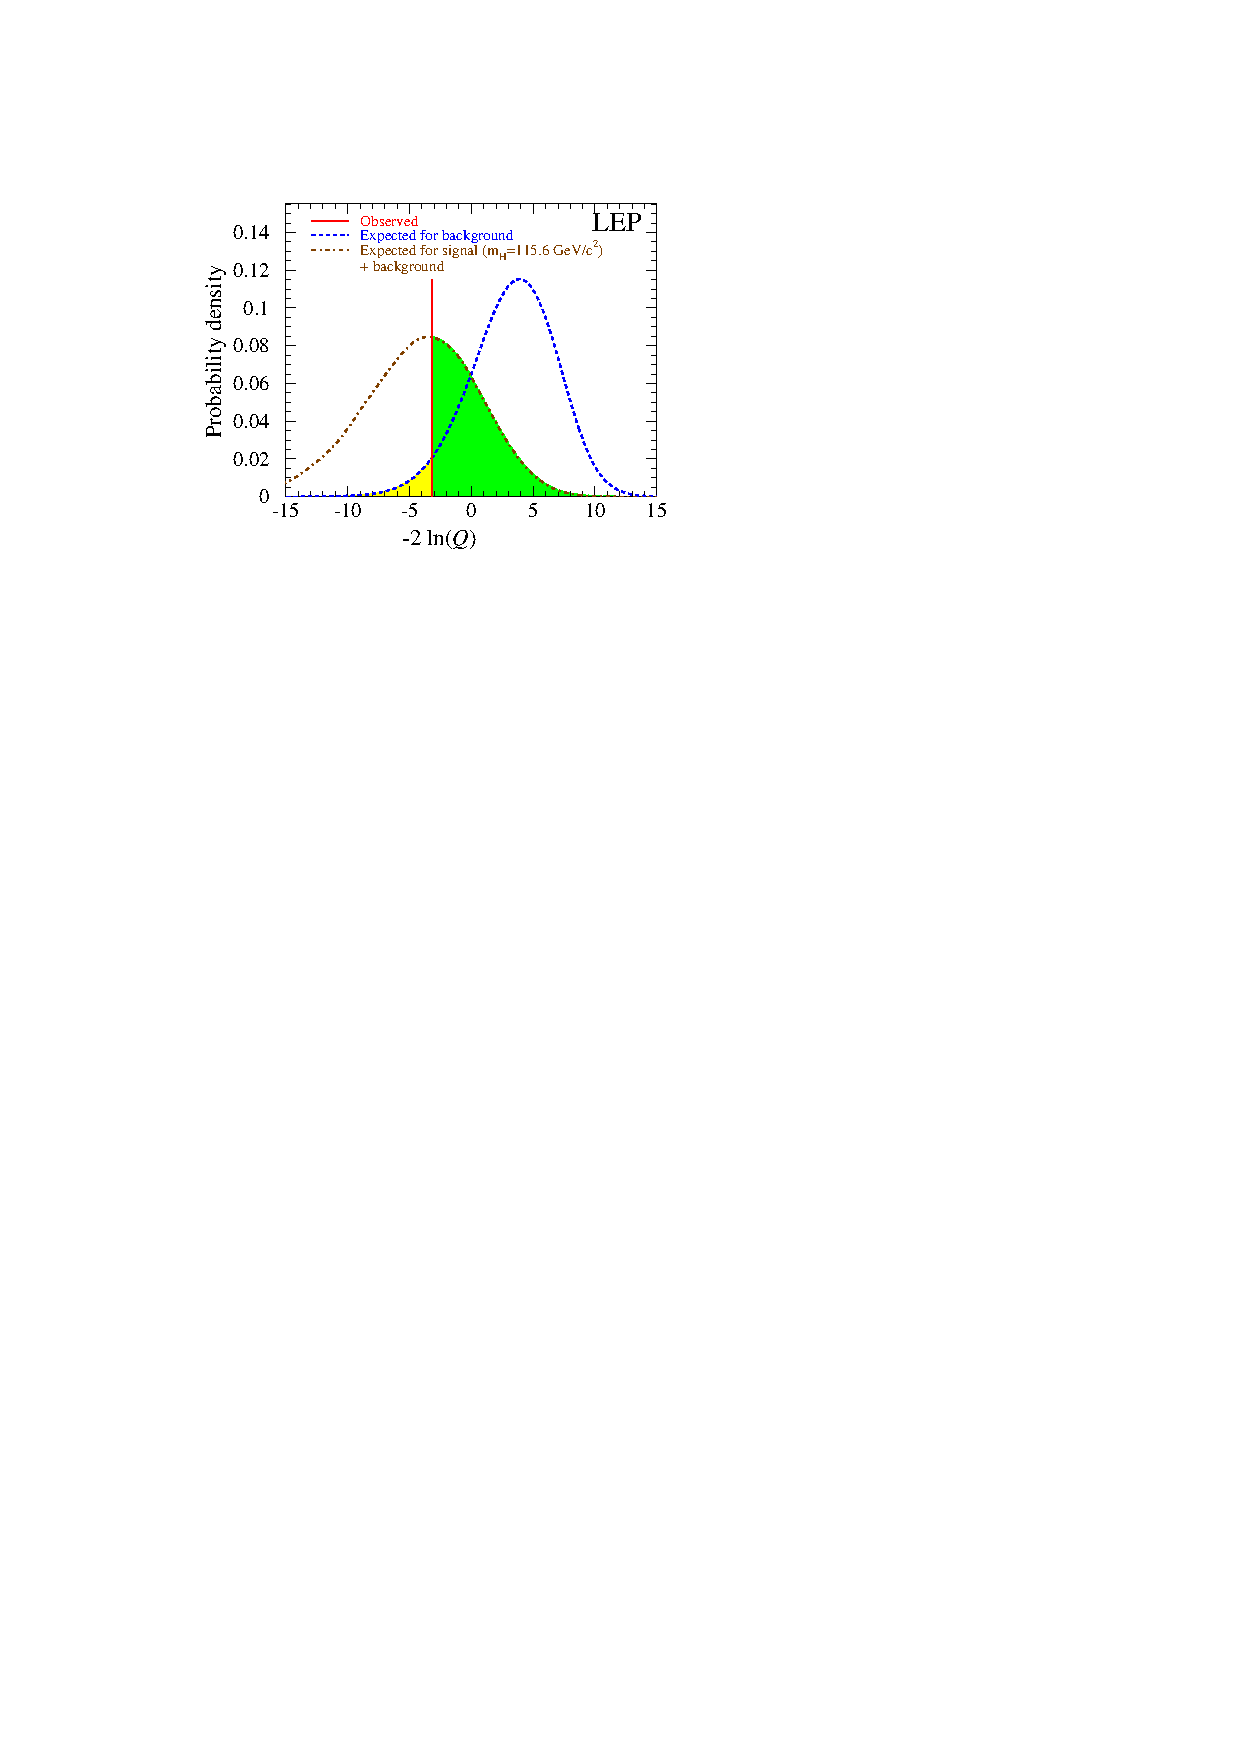
\includegraphics[width=0.95\textwidth]{figures/g21013-fig1.pdf}
\caption{Comparison of the observed value (red line) to the probability densities for $H_{0}$ (background only, blue line) and $H_{1}$ (signal + background, brown line) as a function of the log likelihood ratio. Green area: $CL_{s+b}$, yellow area: $1-CL_{b}$. From \cite{Read:presentation}.}
\label{fig:q}
\end{center}
\end{figure}

We extract a limit on the signal hypothesis by solving $CL_{s}=1-\alpha$ where $\alpha$ is the confidence level, typically 95\%.